\PassOptionsToPackage{unicode=true}{hyperref} % options for packages loaded elsewhere
\PassOptionsToPackage{hyphens}{url}
%
\documentclass[ignorenonframetext,]{beamer}
\usepackage{pgfpages}
\setbeamertemplate{caption}[numbered]
\setbeamertemplate{caption label separator}{: }
\setbeamercolor{caption name}{fg=normal text.fg}
\beamertemplatenavigationsymbolsempty
% Prevent slide breaks in the middle of a paragraph:
\widowpenalties 1 10000
\raggedbottom
\setbeamertemplate{part page}{
\centering
\begin{beamercolorbox}[sep=16pt,center]{part title}
  \usebeamerfont{part title}\insertpart\par
\end{beamercolorbox}
}
\setbeamertemplate{section page}{
\centering
\begin{beamercolorbox}[sep=12pt,center]{part title}
  \usebeamerfont{section title}\insertsection\par
\end{beamercolorbox}
}
\setbeamertemplate{subsection page}{
\centering
\begin{beamercolorbox}[sep=8pt,center]{part title}
  \usebeamerfont{subsection title}\insertsubsection\par
\end{beamercolorbox}
}
\AtBeginPart{
  \frame{\partpage}
}
\AtBeginSection{
  \ifbibliography
  \else
    \frame{\sectionpage}
  \fi
}
\AtBeginSubsection{
  \frame{\subsectionpage}
}
\usepackage{lmodern}
\usepackage{amssymb,amsmath}
\usepackage{ifxetex,ifluatex}
\usepackage{fixltx2e} % provides \textsubscript
\ifnum 0\ifxetex 1\fi\ifluatex 1\fi=0 % if pdftex
  \usepackage[T1]{fontenc}
  \usepackage[utf8]{inputenc}
  \usepackage{textcomp} % provides euro and other symbols
\else % if luatex or xelatex
  \usepackage{unicode-math}
  \defaultfontfeatures{Ligatures=TeX,Scale=MatchLowercase}
\fi
% use upquote if available, for straight quotes in verbatim environments
\IfFileExists{upquote.sty}{\usepackage{upquote}}{}
% use microtype if available
\IfFileExists{microtype.sty}{%
\usepackage[]{microtype}
\UseMicrotypeSet[protrusion]{basicmath} % disable protrusion for tt fonts
}{}
\IfFileExists{parskip.sty}{%
\usepackage{parskip}
}{% else
\setlength{\parindent}{0pt}
\setlength{\parskip}{6pt plus 2pt minus 1pt}
}
\usepackage{hyperref}
\hypersetup{
            pdftitle={Echantillonnage préférentiel},
            pdfauthor={Pierre Gloaguen},
            pdfborder={0 0 0},
            breaklinks=true}
\urlstyle{same}  % don't use monospace font for urls
\newif\ifbibliography
\usepackage{graphicx,grffile}
\makeatletter
\def\maxwidth{\ifdim\Gin@nat@width>\linewidth\linewidth\else\Gin@nat@width\fi}
\def\maxheight{\ifdim\Gin@nat@height>\textheight\textheight\else\Gin@nat@height\fi}
\makeatother
% Scale images if necessary, so that they will not overflow the page
% margins by default, and it is still possible to overwrite the defaults
% using explicit options in \includegraphics[width, height, ...]{}
\setkeys{Gin}{width=\maxwidth,height=\maxheight,keepaspectratio}
\setlength{\emergencystretch}{3em}  % prevent overfull lines
\providecommand{\tightlist}{%
  \setlength{\itemsep}{0pt}\setlength{\parskip}{0pt}}
\setcounter{secnumdepth}{0}

% set default figure placement to htbp
\makeatletter
\def\fps@figure{htbp}
\makeatother

\newcommand{\rmd}{\text{d}}
\newcommand{\R}{\mathbb{R}}
\newcommand{\E}{\mathbb{E}}
\newcommand{\V}{\mathbb{V}}
\newcommand{\Unif}{\mathcal{U}}
\newcommand{\Pro}{\mathbb{P}}
\newcommand{\N}{\mathbb{N}}
\newcommand{\Nor}{\mathcal{N}}
\newcommand{\Cov}{\mathbb{C}\text{ov}}
\newcommand{\I}[1]{\mathbf{1}_{#1}}
\newcommand{\e}[1]{\text{e}^{#1}}
\newcommand{\K}{\mathcal{K}}
\newcommand{\seqN}[1]{\left(#1_n\right)_{n\in\N}}
\makeatletter
\let\save@measuring@true\measuring@true
\def\measuring@true{%
  \save@measuring@true
  \def\beamer@sortzero##1{\beamer@ifnextcharospec{\beamer@sortzeroread{##1}}{}}%
  \def\beamer@sortzeroread##1<##2>{}%
  \def\beamer@finalnospec{}%
}
\makeatother

\title{Echantillonnage préférentiel}
\author{Pierre Gloaguen}
\date{02/04/2020}

\begin{document}
\frame{\titlepage}

\begin{frame}{Annonces:}
\protect\hypertarget{annonces}{}

\begin{itemize}
\tightlist
\item
  Premier rendu pour le 13 Avril (exo5 du TD1)
\item
  À faire en binome (à compléter sur le lien envoyé par mail)
\item
  Corrections des exos 1 à 4 du TD1 mis en ligne
\item
  On regardera ces corrections et vos questions aujourd'hui
\end{itemize}

\end{frame}

\begin{frame}{Rappel de l'épisode précédent}
\protect\hypertarget{rappel-de-luxe9pisode-pruxe9cuxe9dent}{}

\begin{itemize}
\tightlist
\item
  Principes des méthodes de Monte Carlo;
\item
  Approximation d'intégrales (espérances) par simulation;
\item
  Fonctionne grâce à la loi des grands nombres, IC grâce au TCL.
\end{itemize}

\end{frame}

\begin{frame}{Objectif du cours}
\protect\hypertarget{objectif-du-cours}{}

\begin{itemize}
\tightlist
\item
  Présentation de l'échantillonnage préférentiel

  \begin{itemize}
  \tightlist
  \item
    Extension naturelle des méthodes de MC simples;
  \item
    Améliore l'efficacité dans certains cas;
  \item
    Utile quand on ne sait pas simuler selon une loi donnée;\pause
  \end{itemize}
\item
  Motivation: cas de Monte Carlo problématiques;
\item
  Définition;
\item
  Propriétés: Analyse de la variance de ce nouvel estimateur;
\item
  Illustration.
\end{itemize}

\end{frame}

\hypertarget{echantillonnage-pruxe9fuxe9rentiel}{%
\section{Echantillonnage
préférentiel}\label{echantillonnage-pruxe9fuxe9rentiel}}

\begin{frame}{Exemple problématique:}
\protect\hypertarget{exemple-probluxe9matique}{}

On veut calculer
\[I = \mathbb{E}\left[\varphi(X) \right] = \int_{\mathbb{R}}\varphi(x)f(x)\text{d}x\]
où \(X \sim \mathcal{N}(0, 1)\) (de densité \(f(x)\)) et
\[\varphi(x) = \sin^2(x)\text{e}^{-5(x - 5)^2}\]

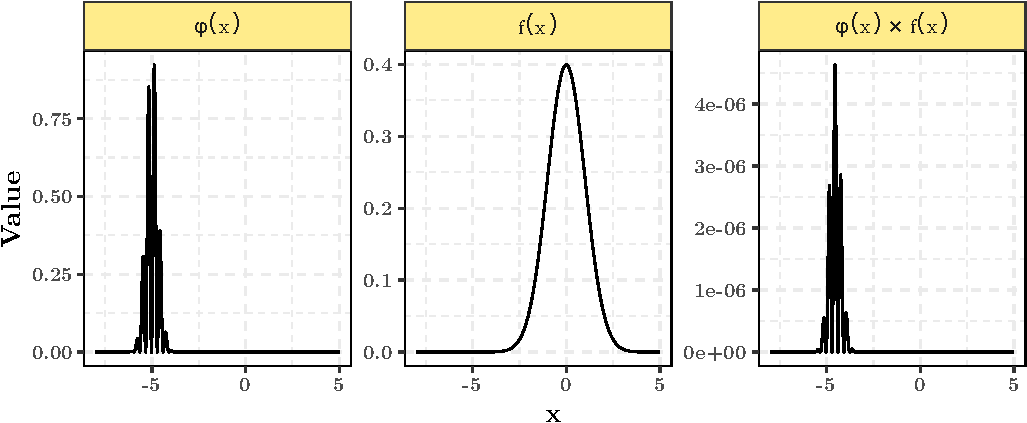
\includegraphics{diapos_importance_sampling_files/figure-beamer/plot_functions-1.pdf}

\end{frame}

\begin{frame}{Estimateur Monte Carlo naturel}
\protect\hypertarget{estimateur-monte-carlo-naturel}{}

On tire \(M = 50000\) points dans une loi \(\mathcal{N}(0, 1)\), et on
calcule la moyenne empirique.

\end{frame}

\begin{frame}{Résultats obtenus:}
\protect\hypertarget{ruxe9sultats-obtenus}{}

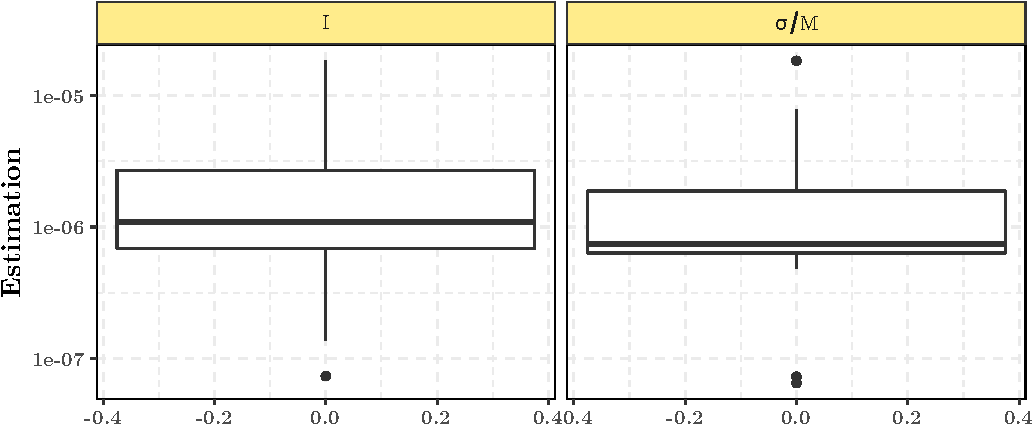
\includegraphics{diapos_importance_sampling_files/figure-beamer/resultats_estimation-1.pdf}

\end{frame}

\begin{frame}{Une trajectoire d'estimation}
\protect\hypertarget{une-trajectoire-destimation}{}

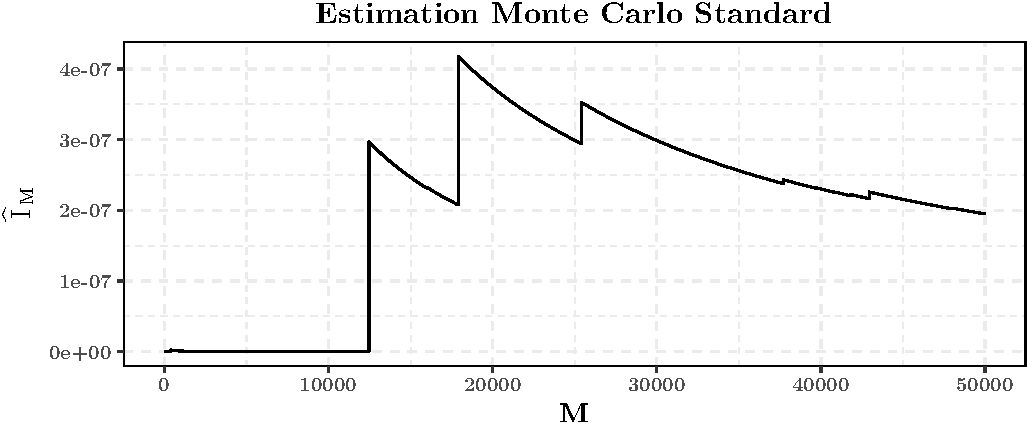
\includegraphics{diapos_importance_sampling_files/figure-beamer/plot_my_mc_estimate-1.pdf}

L'estimation est très instable.

\end{frame}

\begin{frame}{Estimateur Monte Carlo naturel}
\protect\hypertarget{estimateur-monte-carlo-naturel-1}{}

Estimation de la variance et intervalle de confiance asymptotique:

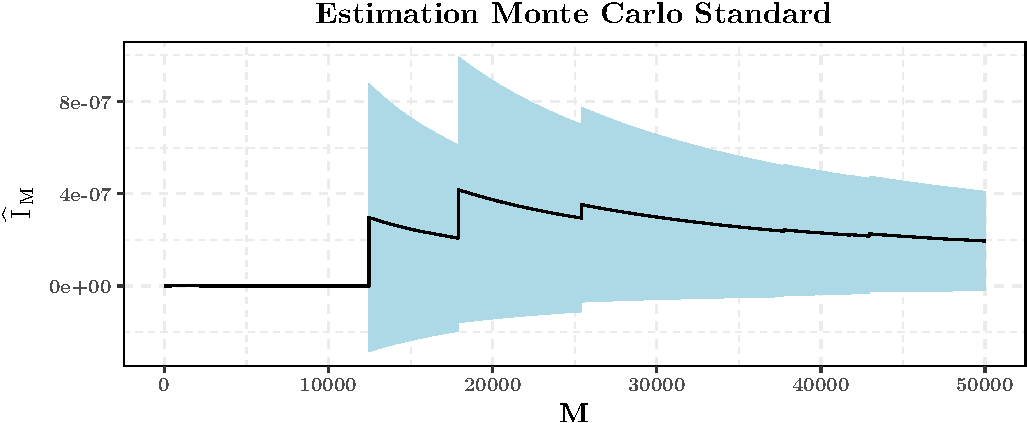
\includegraphics{diapos_importance_sampling_files/figure-beamer/plot_my_mc_estimate_IC-1.pdf}

\end{frame}

\begin{frame}{Manque de chance?}
\protect\hypertarget{manque-de-chance}{}

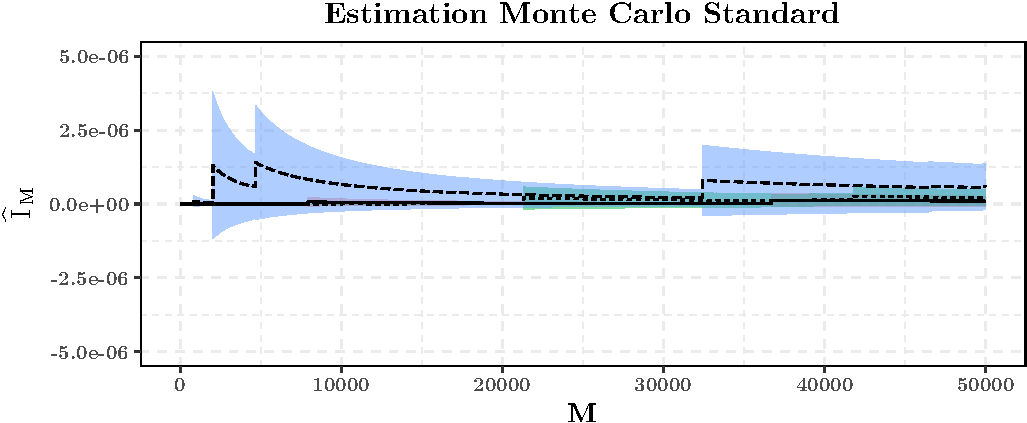
\includegraphics{diapos_importance_sampling_files/figure-beamer/tree_monte_carlo_replicates-1.pdf}

\end{frame}

\begin{frame}{Origine du problème}
\protect\hypertarget{origine-du-probluxe8me}{}

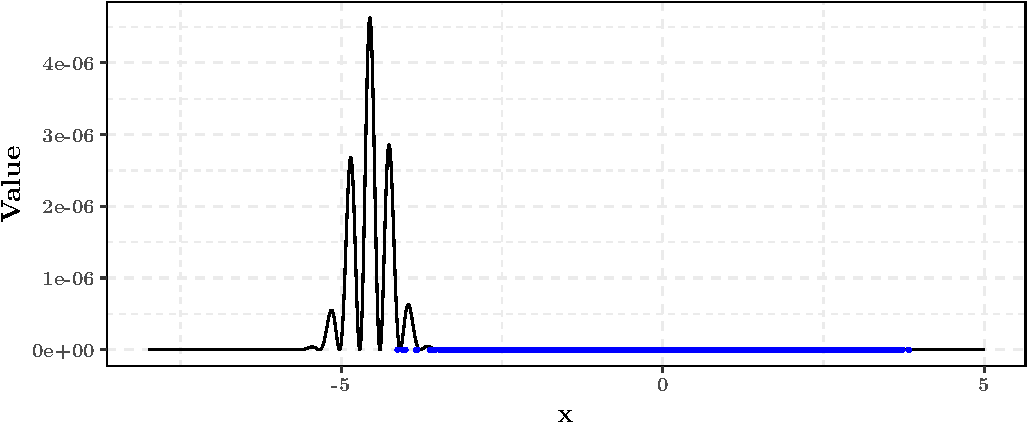
\includegraphics{diapos_importance_sampling_files/figure-beamer/plot_monte_carlo_samples-1.pdf}

On échantillonne loin des régions importantes!

\end{frame}

\begin{frame}{Echantillonnage préférentiel}
\protect\hypertarget{echantillonnage-pruxe9fuxe9rentiel-1}{}

On cherche à estimer une intégrale du type:
\[I = \mathbb{E}_f[\varphi(X)] = \int_{\mathcal{D}_f} \varphi(x) f(x)\rmd x \]
où \(\mathcal{D}_f \subset \R^d\), et \(f\) est une densité de
probabilité sur \(\mathcal{D}_f\) (donc \(f(x) = 0\) pour
\(x \not\in \mathcal{D}_f\)) et \(X\) une v.a. de loi \(f\). \pause

Soit \(g\) une densité de probabilité sur
\(\mathcal{D}_g \supseteq \mathcal{D}_f\) telle que
\(x\in \mathcal{D}_f \Rightarrow g(x) > 0\) et \(Y\) une variable
aléatoire de loi \(g\), alors: \begin{align*}
I &=  \int_{\mathcal{D}_f} \varphi(x) \frac{f(x)}{g(x)}g(x)\rmd x &\\ \pause
&= \int_{\mathcal{D}_g}  \varphi(x) \frac{f(x)}{g(x)}g(x)\rmd x & \text{ as } x \not\in \mathcal{D}_f \Rightarrow f(x) = 0\\ \pause
&= \mathbb{E}_g\left[\varphi(Y) \frac{f(Y)}{g(Y)}\right]&
\end{align*}

\end{frame}

\begin{frame}{Echantillonnage preferentiel}
\protect\hypertarget{echantillonnage-preferentiel}{}

Comme estimateur de \(I\), on peut ainsi proposer l'estimateur:
\[\hat{I}^{IS}_M = \frac{1}{M}\sum_{k = 1}^M \frac{f(Y_k)}{g(Y_k)} \varphi(Y_k)  = \frac{1}{M}\sum_{k = 1}^M W(Y_k)\varphi(Y_k)\]
où \(Y_1,\dots,Y_M\) est un échantillon i.i.d. de variables aléatoires
sur \(\R^d\) de densité \(g\).\pause

\textbf{Remarques:}

\begin{itemize}
\tightlist
\item
  Comme \(Y_k \sim g\), \(g(Y_k)\) est p.s. \(\neq 0\)\pause
\item
  La variable aléatoire \(W(Y_k) = \frac{f(Y_k)}{g(Y_k)}\) est appelée
  \textbf{poids d'importance} de \(Y_k\). \pause
\item
  Quand \(f = g\), on a l'estimateur MC standard (et chaque poids vaut
  1).
\end{itemize}

\end{frame}

\begin{frame}{Quel intérêt?}
\protect\hypertarget{quel-intuxe9ruxeat}{}

On peut choisir \(g\) afin d'échantillonner dans les zones d'importance!

\textbf{Biais:} \begin{align*}
\E_g[\hat{I}^{IS}_M]&=\frac{1}{M}\sum_{k=1}^M\int_{\mathcal{D}_g}  \frac{f(x)}{g(x)}\varphi(x) g(x) \rmd x\\
&=\int_{\mathcal{D}_f}  f(x)\varphi(x) \rmd x = I
\end{align*} Donc, cet estimateur reste sans biais\pause

\textbf{Variance:}
\[\V_g[\hat{I}^{IS}_1] = \left[\E_g[\left(W(Y)\varphi(Y)\right)^2]  - I^2\right] = \int_{\mathcal{D}_g}\frac{\left(\varphi(y)f(y) - Ig(y)\right)^2}{g(y)}\rmd y\]

\begin{itemize}
\tightlist
\item
  La variance peut être très réduite si
  \(g(y) \overset{\approx}{\propto} \varphi(y)f(y)\)!
\item
  Ceci peut guider le choix de \(g\)!
\end{itemize}

\end{frame}

\begin{frame}{Exemple}
\protect\hypertarget{exemple}{}

\(g(x)\) est la densité d'une loi de Student \(\mathcal{T}(3)\).

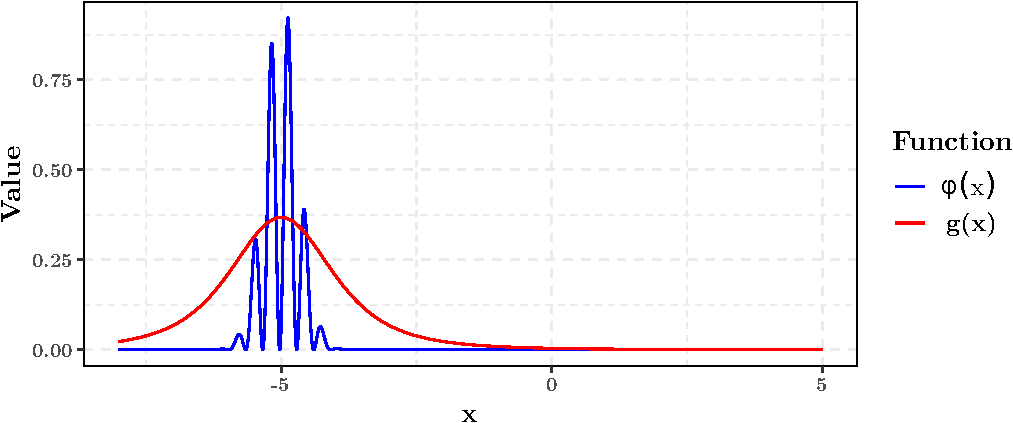
\includegraphics{diapos_importance_sampling_files/figure-beamer/main_plot_is-1.pdf}

\end{frame}

\begin{frame}{Exemple}
\protect\hypertarget{exemple-1}{}

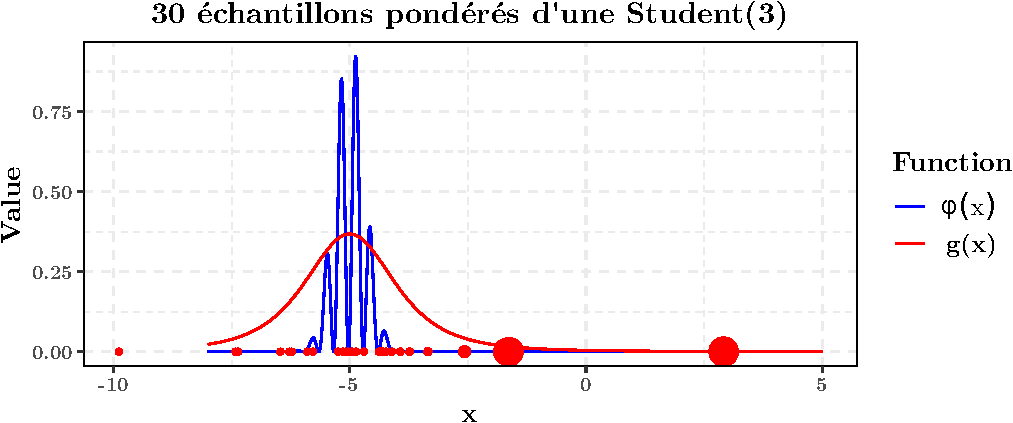
\includegraphics{diapos_importance_sampling_files/figure-beamer/plot_is_estimate_example-1.pdf}

\end{frame}

\begin{frame}{Estimation de \(I\) (et IC asymptotique)}
\protect\hypertarget{estimation-de-i-et-ic-asymptotique}{}

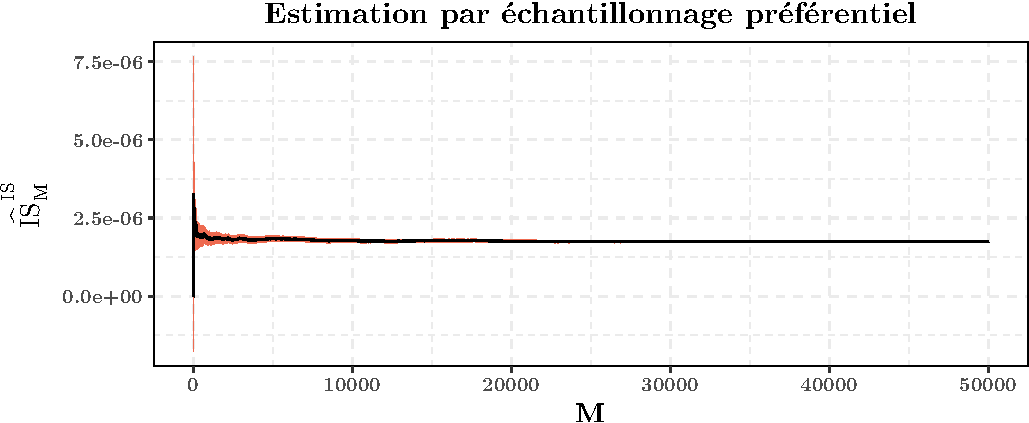
\includegraphics{diapos_importance_sampling_files/figure-beamer/plot_is_estimate-1.pdf}

\end{frame}

\begin{frame}{Comparaison sur cet exemple}
\protect\hypertarget{comparaison-sur-cet-exemple}{}

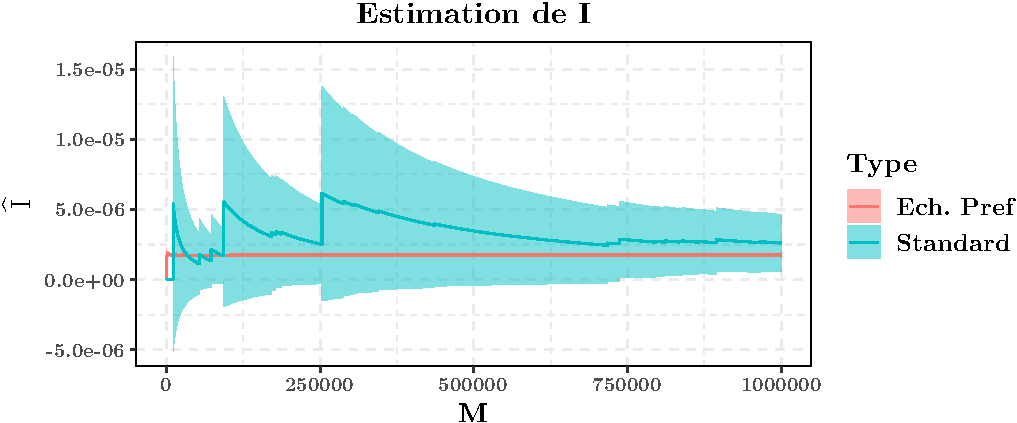
\includegraphics{diapos_importance_sampling_files/figure-beamer/compare_is_mc-1.pdf}

\end{frame}

\begin{frame}{Echantillonnage préférentiel}
\protect\hypertarget{echantillonnage-pruxe9fuxe9rentiel-2}{}

\begin{block}{Avantages}

\begin{itemize}
\tightlist
\item
  Très utile pour l'estimation de quantités petites (probabilités
  d'évènements rares). \pause
\item
  Peut amener à une forte réduction de variance \pause
\item
  Peut aussi être utiliser quand on ne sait pas simuler selon \(f\)!
  \pause
\end{itemize}

\end{block}

\begin{block}{Attention!}

\begin{itemize}
\tightlist
\item
  Nécessite le choix de \(g\)! Pas toujours évident (notamment en grande
  dimension)!\pause
\item
  Un mauvais \(g\) peut amener à un estimateur de variance infinie!
  (voir TD).
\item
  Un bon choix de \(g\) est souvent ``problème dépendant'', (ne
  conviendra que pour \(\E[\varphi(X)]\) pour un \(\varphi\)
  spécifique).
\end{itemize}

\end{block}

\end{frame}

\hypertarget{echantillonnage-pruxe9fuxe9rentiel-normalisuxe9}{%
\section{Echantillonnage préférentiel
normalisé}\label{echantillonnage-pruxe9fuxe9rentiel-normalisuxe9}}

\begin{frame}{Problématique}
\protect\hypertarget{probluxe9matique}{}

Objectif, calculer:
\[I = \mathbb{E}[\varphi(X)] = \int_{\mathcal{D}_f} \varphi(x) f(x) d(x)\]

Supposons que \(f\) ne soit connue qu'à une constante près:
\[f(x) = \frac{\overbrace{f^{(u)}(x)}^{\text{Connu}}}{\underbrace{\int_{\mathcal{D}_f} f^{(u)}(z)\rmd z}_\text{Inconnu}}.\]

\begin{itemize}
\item
  Pour une densité de proposition \(g\), on ne peut plus calculer le
  poids d'importance!\pause
\item
  Ce cas est en pratique très fréquent en inférence bayésienne!
\end{itemize}

\end{frame}

\begin{frame}{Echantillonnage préférentiel normalisé}
\protect\hypertarget{echantillonnage-pruxe9fuxe9rentiel-normalisuxe9-1}{}

Si on dispose d'une loi de proposition \(g\) et de \(Y_1,\dots, Y_M\)
tirés indépendemment selon \(g\), alors l'estimateur:
\[\hat{I}^{IS,u}_M = \sum_{k = 1}^M  \frac{f^{(u)}(Y_k)/g(Y_k)}{\sum_{\ell = 1}^M f^{(u)}(Y_\ell) / g(Y_\ell)}\varphi(Y_k)\]
est un estimateur consistant (convergence en proba.) de \(I\).\pause

\begin{itemize}
\tightlist
\item
  Estimateur biaisé pour \(M\) petit;
\item
  Peut amener à un estimateur de variance plus faible que
  l'échantillonnage préférentiel classique.
\end{itemize}

\end{frame}

\begin{frame}{Autres méthodes de réduction de variance}
\protect\hypertarget{autres-muxe9thodes-de-ruxe9duction-de-variance}{}

\begin{itemize}
\tightlist
\item
  Conditionnement
\item
  Variables de contrôles
\item
  Quasi Monte Carlo
\end{itemize}

Voir références dans le poly.

\end{frame}

\end{document}
